\documentclass[10pt,letterpaper]{article}
\usepackage[top=1in,bottom=1in,left=1in,right=1in]{geometry}
\usepackage{datetime}
\usepackage{natbib}      % http://merkel.zoneo.net/Latex/natbib.php
\usepackage{palatino}
\usepackage{verbatim}
\usepackage[normalem]{ulem}
\bibpunct{(}{)}{;}{a}{,}{,}

\usepackage{array}

\usepackage{chngpage}
\usepackage{stmaryrd}
\usepackage{amssymb}
\usepackage{amsmath}
\usepackage{graphicx}
\usepackage{lscape}
\usepackage{subfigure}
\usepackage[usenames,dvipsnames]{color}
\definecolor{myblue}{rgb}{0,0.1,0.6}
\definecolor{mygreen}{rgb}{0,0.3,0.1}
\usepackage[colorlinks=true,linkcolor=black,citecolor=mygreen,urlcolor=myblue]{hyperref}

\newcommand{\bocomment}[1]{\textcolor{Bittersweet}{BO says: #1}}

\newcommand{\ignore}[1]{}
\newcommand{\transpose}{^\mathsf{T}}
\newcommand{\inner}[1]{\langle #1 \rangle} 
\newcommand{\smallsec}[1]{\noindent \textbf{#1\ }}
\newcommand{\cmd}[1] {{\color{blue}\texttt{#1}}}

\newcommand{\solution}[1]{{\color{myblue} \emph{[Solution:} 

#1 

\emph{End solution]}}}
\newcommand{\solutionnote}[1]{{\color{myblue} \emph{[Note:}

#1 

\emph{End note]}}}
\newcommand{\points}[1]{{\color{mygreen}\emph{[#1]\ \ }}}

\newcommand{\aone}{\diamondsuit}
\newcommand{\atwo}{\heartsuit}
\newcommand{\bone}{\triangle}
\newcommand{\btwo}{\Box}
\newcommand{\myand}{\ \land\ }
\newcommand{\myor}{\ \lor\ }
\newcommand{\mynot}{\lnot}

\title{
  \textbf{Mini-project 1: Color images Solution} \\
  \textbf{Name: Abhay Doke}\\
  \textbf{UID:29552668}
}

\settimeformat{ampmtime}
\date{}
\begin{document}
\maketitle

\section{Aligning Prokudin-Gorskii images - Aligned output images} 
For aligning the Prokudin-Gorskii images I have used their edge information for calculating Sum of Squared Differences (SSD) distances.
Edge information is preserved  
All the images can be found in the "output/prokudin-gorskii/" folder.

\begin{figure}[h]
\centering
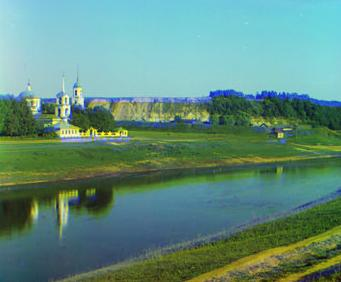
\includegraphics[width=0.5\textwidth]{output/prokudin-gorskii/00125-aligned.jpg}
\caption{00125-aligned.jpg}
\end{figure}

\begin{figure}[h]
\centering
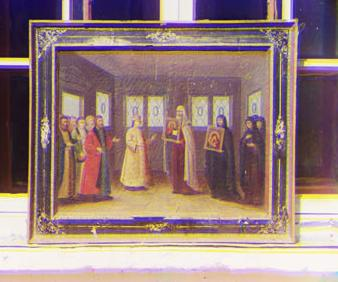
\includegraphics[width=0.5\textwidth]{output/prokudin-gorskii/00149-aligned.jpg}
\caption{00149-aligned.jpg}
\end{figure}

\begin{figure}[h]
\centering
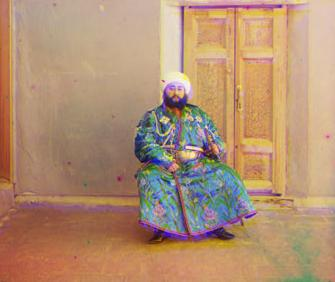
\includegraphics[width=0.5\textwidth]{output/prokudin-gorskii/00153-aligned.jpg}
\caption{00153-aligned.jpg}
\end{figure}

\begin{figure}[h]
\centering
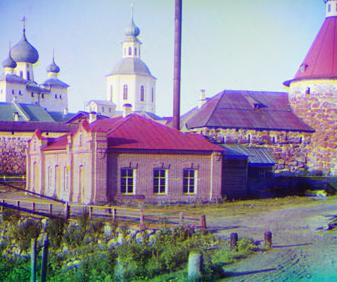
\includegraphics[width=0.5\textwidth]{output/prokudin-gorskii/00351-aligned.jpg}
\caption{00351-aligned.jpg}
\end{figure}

\begin{figure}[h]
\centering
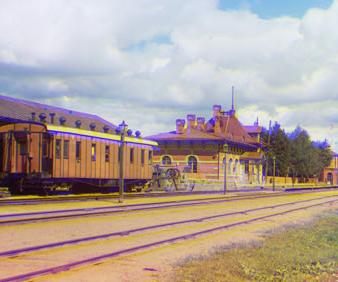
\includegraphics[width=0.5\textwidth]{output/prokudin-gorskii/00398-aligned.jpg}
\caption{00398-aligned.jpg}
\end{figure}

\begin{figure}[h]
\centering
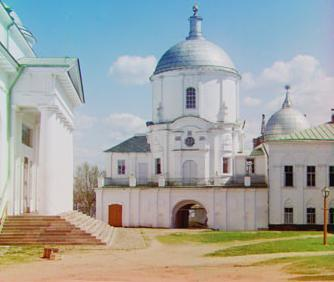
\includegraphics[width=0.5\textwidth]{output/prokudin-gorskii/01112-aligned.jpg}
\caption{01112-aligned.jpg}
\end{figure}



























\end{document}